%% v4_arch.tex — V4 multimodal architecture diagram (compact horizontal layout)
%% Rendered via \resizebox{\textwidth}{!}{\input{...}} inside figure*

\usetikzlibrary{positioning, arrows.meta, calc, fit, backgrounds, shapes.geometric, shapes.misc}

%% ── Colour definitions (muted academic palette) ──────────────────────────────
\definecolor{S1Blue}{RGB}{52,100,158}
\definecolor{S1BgCol}{RGB}{232,240,252}
\definecolor{S1Bdr}{RGB}{110,150,200}

\definecolor{BranchACol}{RGB}{180,100,30}
\definecolor{BranchABg}{RGB}{253,245,228}
\definecolor{BranchABdr}{RGB}{200,140,60}

\definecolor{BranchBCol}{RGB}{38,120,90}
\definecolor{BranchBBg}{RGB}{228,248,238}
\definecolor{BranchBBdr}{RGB}{70,160,110}

\definecolor{FuseCol}{RGB}{130,30,50}
\definecolor{FuseBg}{RGB}{250,232,236}
\definecolor{FuseBdr}{RGB}{175,60,80}

\definecolor{IOCol}{RGB}{60,60,70}
\definecolor{IOBg}{RGB}{240,240,244}

\definecolor{AuxCol}{RGB}{185,40,40}
\definecolor{AuxBg}{RGB}{255,238,238}

\definecolor{ShapeCol}{RGB}{80,80,95}
\definecolor{StageLbl}{RGB}{40,40,55}

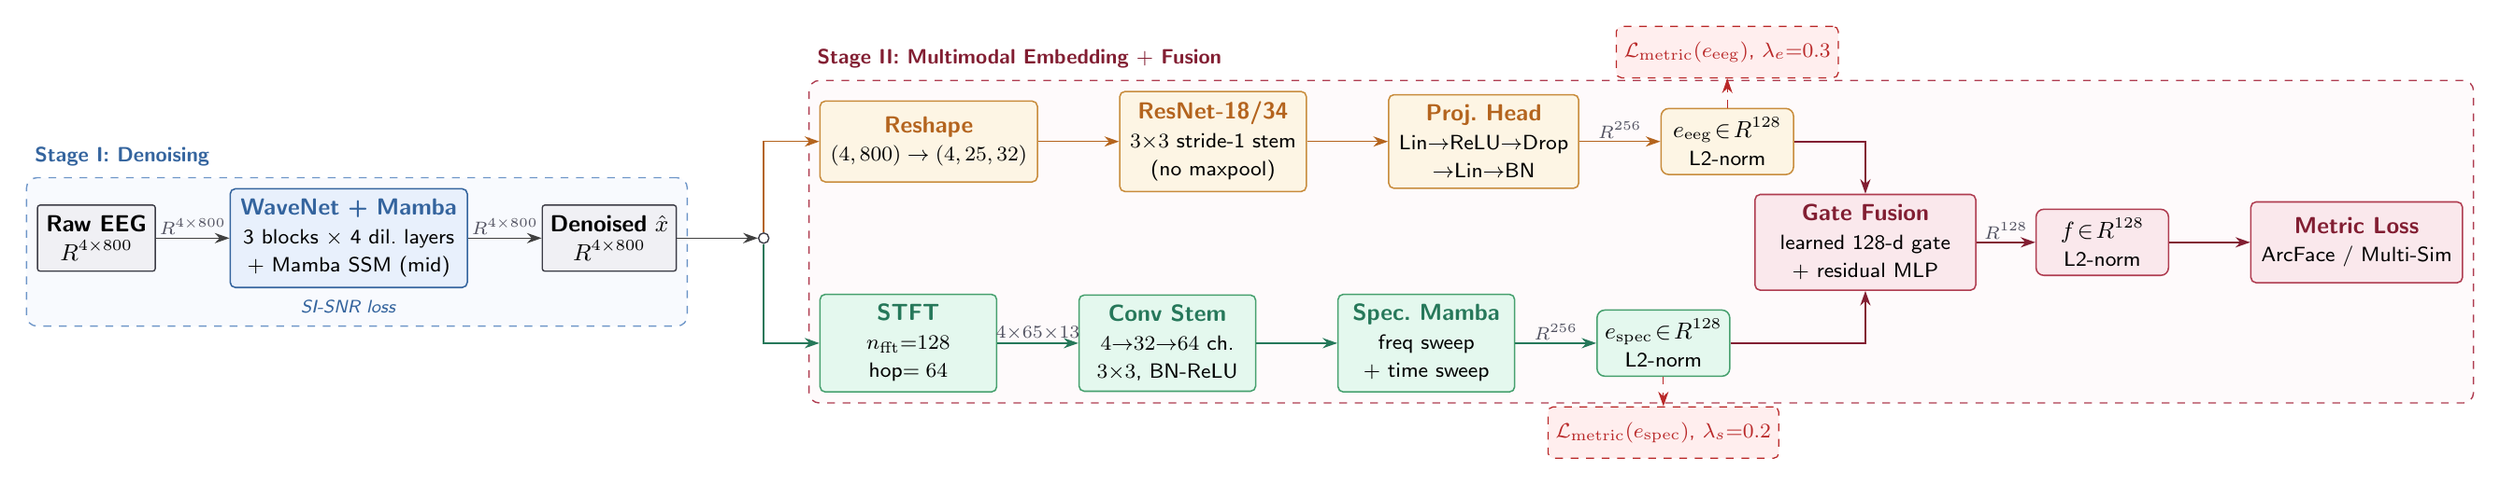
\begin{tikzpicture}[
    font=\small\sffamily,
    node distance=5mm and 7mm,
    >={Stealth[length=2.0mm, width=1.4mm]},
    every node/.style={align=center},
    blk/.style={
        draw, rounded corners=2pt,
        inner sep=4pt, minimum height=11mm,
        line width=0.55pt
    },
    ionode/.style={
        draw=IOCol, fill=IOBg, rounded corners=1pt,
        inner sep=3pt, minimum height=9mm, minimum width=16mm,
        line width=0.5pt, font=\small\sffamily
    },
    s1blk/.style={blk, draw=S1Blue, fill=S1BgCol, minimum width=27mm},
    ablk/.style={blk, draw=BranchABdr, fill=BranchABg, minimum width=24mm},
    bblk/.style={blk, draw=BranchBBdr, fill=BranchBBg, minimum width=24mm},
    fblk/.style={blk, draw=FuseBdr, fill=FuseBg, minimum width=30mm},
    embnode/.style={
        draw, rounded corners=3pt,
        inner sep=3pt, minimum height=9mm, minimum width=18mm,
        line width=0.55pt
    },
    auxblk/.style={
        draw=AuxCol, fill=AuxBg, dashed,
        rounded corners=2pt,
        inner sep=3pt, minimum height=7mm, minimum width=22mm,
        line width=0.45pt, font=\footnotesize\sffamily
    },
    splitnode/.style={
        circle, draw=IOCol, fill=white,
        inner sep=0pt, minimum size=4pt,
        line width=0.5pt
    },
    fl/.style={->, line width=0.5pt, draw=black!75},
    flA/.style={->, line width=0.5pt, draw=BranchACol},
    flB/.style={->, line width=0.5pt, draw=BranchBCol},
    flF/.style={->, line width=0.6pt, draw=FuseCol},
    auxfl/.style={->, dashed, line width=0.4pt, draw=AuxCol},
    tlbl/.style={font=\scriptsize\itshape\sffamily, text=ShapeCol, inner sep=1pt},
    losslbl/.style={font=\scriptsize\sffamily, text=S1Blue, inner sep=1pt},
    auxlbl/.style={font=\scriptsize\sffamily, text=AuxCol, inner sep=1pt},
]

%% ═══════════════════════════════════════════════════════════════════════════
%%   [Input]──[Denoiser]──[Denoised]──●──┬──[Reshape]──[ResNet]──[ProjH]──[e_eeg]──┐
%%                                       │                                          ├──[Fusion]──[f]──[Loss]
%%                                       └──[STFT]──[ConvStem]──[SpecMamba]──[e_spec]┘
%% ═══════════════════════════════════════════════════════════════════════════

%% ── Stage I: input → denoiser → denoised ──
\node[ionode] (input) {%
    \textbf{Raw EEG}\\
    $\mathbb{R}^{4\times 800}$%
};

\node[s1blk, right=10mm of input] (denoiser) {%
    \textcolor{S1Blue}{\textbf{WaveNet + Mamba}}\\
    \footnotesize 3 blocks $\times$ 4 dil.\ layers\\
    \footnotesize + Mamba SSM (mid)%
};
\node[losslbl, below=1.2mm of denoiser] (sisnrlbl) {\textit{SI-SNR loss}};

\node[ionode, right=10mm of denoiser] (denoised) {%
    \textbf{Denoised} $\hat{x}$\\
    $\mathbb{R}^{4\times 800}$%
};

\node[splitnode, right=11mm of denoised] (split) {};

%% ── Branch A (upper): ResNet EEG embedder ──
\node[ablk, above right=7mm and 7mm of split] (reshape) {%
    \textcolor{BranchACol}{\textbf{Reshape}}\\
    \footnotesize $(4,800)\to(4,25,32)$%
};

\node[ablk, right=11mm of reshape] (resnet) {%
    \textcolor{BranchACol}{\textbf{ResNet-18/34}}\\
    \footnotesize $3{\times}3$ stride-1 stem\\
    \footnotesize (no maxpool)%
};

\node[ablk, right=11mm of resnet] (projhead) {%
    \textcolor{BranchACol}{\textbf{Proj.\ Head}}\\
    \footnotesize Lin$\to$ReLU$\to$Drop\\
    \footnotesize $\to$Lin$\to$BN%
};

\node[embnode, draw=BranchABdr, fill=BranchABg, right=11mm of projhead] (eegemb) {%
    $e_{\mathrm{eeg}}\!\in\!\mathbb{R}^{128}$\\
    \footnotesize L2-norm%
};

%% ── Branch B (lower): Spectrogram Mamba ──
\node[bblk, below right=7mm and 7mm of split] (stft) {%
    \textcolor{BranchBCol}{\textbf{STFT}}\\
    \footnotesize $n_{\mathrm{fft}}{=}128$\\
    \footnotesize hop$=64$%
};

\node[bblk, right=11mm of stft] (convstem) {%
    \textcolor{BranchBCol}{\textbf{Conv Stem}}\\
    \footnotesize $4{\to}32{\to}64$ ch.\\
    \footnotesize $3{\times}3$, BN-ReLU%
};

\node[bblk, right=11mm of convstem] (specmamba) {%
    \textcolor{BranchBCol}{\textbf{Spec.\ Mamba}}\\
    \footnotesize freq sweep\\
    \footnotesize $+$ time sweep%
};

\node[embnode, draw=BranchBBdr, fill=BranchBBg, right=11mm of specmamba] (specemb) {%
    $e_{\mathrm{spec}}\!\in\!\mathbb{R}^{128}$\\
    \footnotesize L2-norm%
};

%% ── Fusion (vertically centred between embeddings) ──
\node[fblk] at ($(eegemb.east)!0.5!(specemb.east) + (14mm,0)$) (fusion) {%
    \textcolor{FuseCol}{\textbf{Gate Fusion}}\\
    \footnotesize learned 128-d gate\\
    \footnotesize $+$ residual MLP%
};

\node[embnode, draw=FuseBdr, fill=FuseBg, right=8mm of fusion] (fout) {%
    $f\!\in\!\mathbb{R}^{128}$\\
    \footnotesize L2-norm%
};

\node[fblk, right=11mm of fout, minimum width=24mm] (mainloss) {%
    \textcolor{FuseCol}{\textbf{Metric Loss}}\\
    \footnotesize ArcFace / Multi-Sim%
};

%% ── Auxiliary loss boxes (sit just outside the branches, kept compact) ──
\node[auxblk, above=4mm of eegemb] (auxeeg) {%
    \textcolor{AuxCol}{$\mathcal{L}_{\mathrm{metric}}(e_{\mathrm{eeg}})$, $\lambda_e{=}0.3$}%
};

\node[auxblk, below=4mm of specemb] (auxspec) {%
    \textcolor{AuxCol}{$\mathcal{L}_{\mathrm{metric}}(e_{\mathrm{spec}})$, $\lambda_s{=}0.2$}%
};

%% ═══════════════════════════════════════════════════════════════════════════
%% ARROWS
%% ═══════════════════════════════════════════════════════════════════════════

\draw[fl] (input) -- node[tlbl, above] {$\mathbb{R}^{4\times800}$} (denoiser);
\draw[fl] (denoiser) -- node[tlbl, above] {$\mathbb{R}^{4\times800}$} (denoised);
\draw[fl] (denoised) -- (split);

%% Split → Branch A
\draw[flA] (split) |- (reshape.west);
\draw[flA] (reshape) -- (resnet);
\draw[flA] (resnet)  -- (projhead);
\draw[flA] (projhead) -- node[tlbl, above] {$\mathbb{R}^{256}$} (eegemb);

%% Split → Branch B
\draw[flB] (split) |- (stft.west);
\draw[flB] (stft)     -- node[tlbl, above] {$4{\times}65{\times}13$} (convstem);
\draw[flB] (convstem) -- (specmamba);
\draw[flB] (specmamba) -- node[tlbl, above] {$\mathbb{R}^{256}$} (specemb);

%% Both embeddings → fusion (enter from top/bottom to avoid crossing through box)
\draw[flF] (eegemb.east)  -| (fusion.north);
\draw[flF] (specemb.east) -| (fusion.south);

%% Fusion → output → loss
\draw[flF] (fusion) -- node[tlbl, above] {$\mathbb{R}^{128}$} (fout);
\draw[flF] (fout)   -- (mainloss);

%% Auxiliary loss arrows
\draw[auxfl] (eegemb.north)  -- (auxeeg.south);
\draw[auxfl] (specemb.south) -- (auxspec.north);

%% ═══════════════════════════════════════════════════════════════════════════
%% BACKGROUND STAGE BOXES (aux losses excluded — they sit visually outside)
%% ═══════════════════════════════════════════════════════════════════════════
\begin{pgfonlayer}{background}

    \node[
        draw=S1Bdr, dashed, rounded corners=4pt,
        fill=S1BgCol, fill opacity=0.30,
        line width=0.5pt,
        fit=(input)(denoiser)(denoised)(sisnrlbl),
        inner sep=4pt
    ] (stage1box) {};

    \node[
        draw=FuseBdr, dashed, rounded corners=4pt,
        fill=FuseBg, fill opacity=0.20,
        line width=0.5pt,
        fit=(reshape)(resnet)(projhead)(eegemb)
            (stft)(convstem)(specmamba)(specemb)
            (fusion)(fout)(mainloss),
        inner sep=4pt
    ] (stage2box) {};

\end{pgfonlayer}

%% Stage labels — placed inside top-left of each box, small caps
\node[
    font=\footnotesize\bfseries\sffamily,
    text=S1Blue,
    above=1pt of stage1box.north west,
    anchor=south west
] {\textsc{Stage I}: Denoising};

\node[
    font=\footnotesize\bfseries\sffamily,
    text=FuseCol,
    above=1pt of stage2box.north west,
    anchor=south west
] {\textsc{Stage II}: Multimodal Embedding $+$ Fusion};

\end{tikzpicture}
